\chapter{Szczegóły implementacyjne}

\section{Technologie}
\label{sec:technologies}
W tej sekcji omówiono technologie wykorzystane w projekcie.

Aplikacja została napisana w języku programowania Python. Technologia ta została wybrana ze względu na szeroki wachlarz dostępnych bibliotek, frameworków oraz narzędzi. Doskonale nadaje się do tworzenia aplikacji wykorzystujących techniki uczenia maszynowego. Zainstalowana wersja to \textbf{Python 3.12.6}. Implementacja korzysta z następujących bibliotek:

Aby zmienić wszystkie wystąpienia \texttt na \textbf w podanym tekście, wystarczy zamienić każde \texttt na \textbf. Oto poprawiony tekst:

\begin{itemize}
	\item \textbf{tensorflow} to wszechstronna biblioteka używana do budowy modeli uczenia maszynowego i głębokiego uczenia. Oferuje szerokie wsparcie dla sieci neuronowych, takich jak CNN i RNN. W projekcie została wykorzystana do implementacji zaawansowanych modeli uczenia maszynowego. \textbf{Użyta wersja: '2.18.0'}.
	\item \textbf{keras} jest wysokopoziomowym API opartym na TensorFlow, ułatwiającym budowę i trenowanie modeli głębokiego uczenia. W projekcie została wykorzystana do definiowania warstw, architektury sieci i przygotowania modeli. \textbf{Użyta wersja: '3.6.0'}.
	\item \textbf{scikit-learn} zawiera szeroką gamę narzędzi do uczenia maszynowego, w tym modele klasyfikacji, regresji, klasteryzacji, a także metody wstępnego przetwarzania danych. W projekcie była używana do transformacji danych i budowy modeli klasyfikacyjnych. \textbf{Użyta wersja: '1.5.2'}.
	\item \textbf{xgboost} to wydajna biblioteka do gradientowego zwiększania liczby drzew, szczególnie skuteczna w zadaniach klasyfikacyjnych i regresyjnych. W projekcie została wykorzystana do tworzenia modeli zespołowych. \textbf{Użyta wersja: '2.1.2'}.
	\item \textbf{pandas} to biblioteka przeznaczona do manipulacji danymi i analizy. Ułatwia obsługę dużych zbiorów danych w formie tabelarycznej. W projekcie używana była do wczytywania, czyszczenia i przekształcania danych. \textbf{Użyta wersja: '2.2.3'}.
	\item \textbf{numpy} to podstawowa biblioteka do obliczeń numerycznych w Pythonie. Dostarcza funkcje do operacji na wielowymiarowych tablicach, generowania liczb losowych oraz wykonywania obliczeń matematycznych. \textbf{Użyta wersja: '1.26.4'}.
	\item \textbf{matplotlib} to biblioteka służąca do wizualizacji danych w postaci wykresów i diagramów. W projekcie była używana do przedstawienia wyników w postaci graficznej. \textbf{Użyta wersja: '3.9.2'}.
	\item \textbf{seaborn} to rozszerzenie dla \textbf{matplotlib}, które umożliwia tworzenie bardziej atrakcyjnych i zaawansowanych wizualizacji statystycznych. W projekcie była używana do generowania szczegółowych wykresów danych. \textbf{Użyta wersja: '0.13.2'}.
	\item \textbf{transformers} to biblioteka rozwijana przez Hugging Face, używana do przetwarzania języka naturalnego (NLP). Zawiera zaimplementowane modele, takie jak BERT, GPT, i RoBERTa. W projekcie wykorzystano ją do klasyfikacji tekstu. \textbf{Użyta wersja: '4.46.2'}.
	\item \textbf{torch} (PyTorch) to elastyczna biblioteka do głębokiego uczenia, wspierająca dynamiczne definiowanie sieci neuronowych. W projekcie była używana do tworzenia modeli opartych na sieciach neuronowych i obliczeń tensorowych. \textbf{Użyta wersja: '2.5.1'}.
\end{itemize}

\section{Wymagania systemowe}
\subsection{Sprzęt}
W poniższej podsekcji wymieniono minimalne wymagania sprzętowe do uruchomienia aplikacji i testów.

\begin{itemize}
	\item Procesor: co najmniej 4 rdzenie, 8 wątków, częstotliwość bazowa 3,60 GHz i 6 MB pamięci cache. W testach wykorzystano procesor Intel® CoreTM i7 10700f.
	\item Pamięć: co najmniej 16 GB RAM.
	\item Karta graficzna: dedykowany układ graficzny z co najmniej 4 GB pamięci. W testach wykorzystano AMD® Radeon RX 6400 (4 GB).
	\item Dysk: 4,5 GB wolnej przestrzeni na dysku.
\end{itemize}

\subsection{Oprogramowanie}

Poniżej wymieniono minimalne wymagania dotyczące oprogramowania, niezbędne do uruchomienia aplikacji i testów.

\begin{itemize}
	\item Zainstalowany Python (wersja określona w Sekcji \ref{sec:technologies}).
	\item Zainstalowana najnowsza wersja pip.
	\item Instalacja bibliotek i frameworków odbywa się za pomocą pliku \texttt{requirements.txt}. Aby zainstalować wszystkie wymagane zależności, należy w terminalu uruchomić polecenie \texttt{pip install -r requirements.txt}.
	\item Umieszczenie danych testowych w odpowiednim podfolderze projektu:
	      \texttt{projekt\textbackslash\allowbreak datasets\textbackslash\allowbreak nazwa}. Są dostępne tylko podane trzy opcje datasetów: \textbf{WELFake\_dataset}, \textbf{ISOT\_dataset} oraz \textbf{BuzzFeed\_dataset}.
	      Dane testowe powinny być zapisane w plikach CSV o następującej strukturze:

	      \begin{itemize}
		      \item Kolumny: \texttt{title}, \texttt{text}, \texttt{subject}, \texttt{date}.
	      \end{itemize}
	\item W folderze każdego datasetu powinny znajdować się dwa pliki danych:
	      \begin{itemize}
		      \item \texttt{Fake.csv} - zawierający fałszywe wiadomości.
		      \item \texttt{True.csv} - zawierający prawdziwe wiadomości.
	      \end{itemize}
	\item Wystarczająca ilość miejsca na dane.
\end{itemize}

\section{Architektura Systemu}
System został zaprojektowany do analizy i klasyfikacji tekstów wiadomości jako fałszywe lub prawdziwe, wykorzystując różnorodne algorytmy uczenia maszynowego oraz techniki ensemble. Składa się z czterech głównych warstw, które odpowiadają za przetwarzanie danych, trenowanie modeli, ocenę ich skuteczności oraz wizualizację wyników. Poniżej przedstawiono szczegóły każdej warstwy. Całośc jest pokazana na rysunku \ref{fig:diagram_architekture}.

\begin{figure}[H]
	\centering
	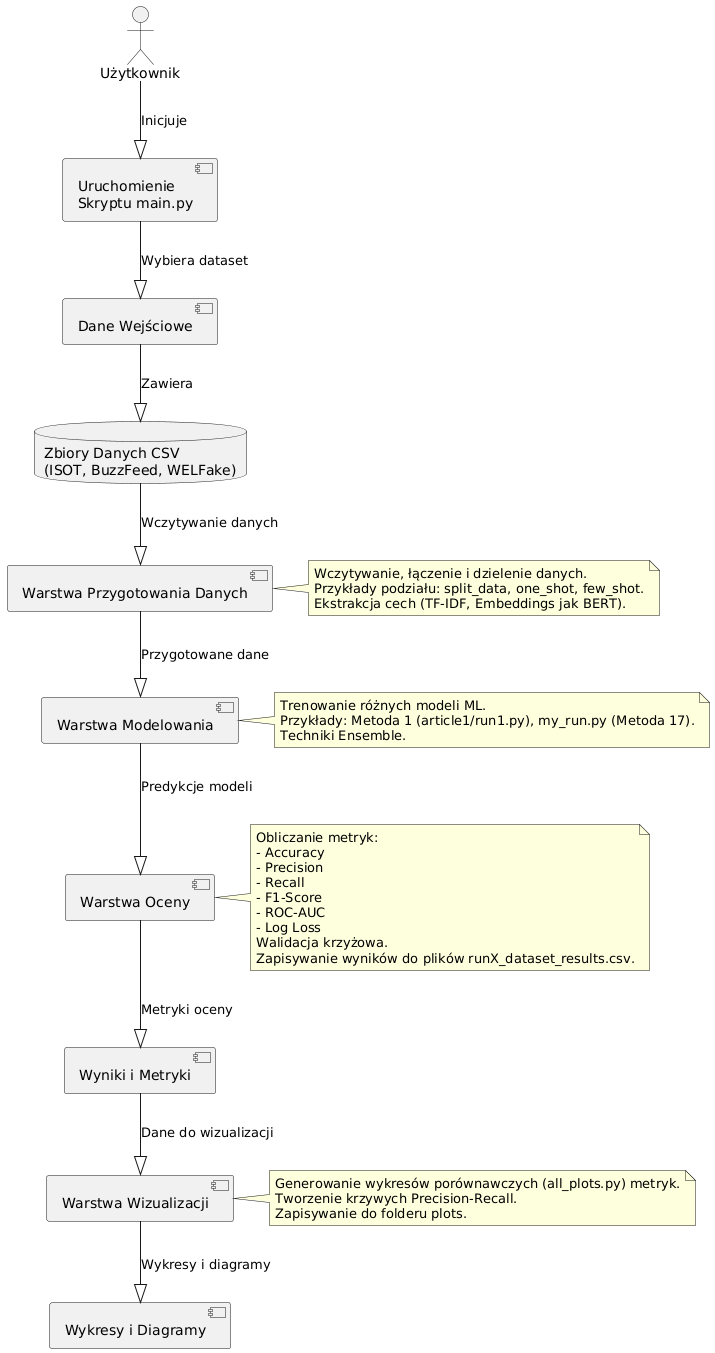
\includegraphics[width=0.6\textwidth]{img/app/SystemArchitecture.png}
	\caption{Diagram architektury systemu.}
	\label{fig:diagram_architekture}
\end{figure}

\subsection{Warstwa Przygotowania Danych}
Dane wejściowe są wczytywane z plików CSV: \texttt{Fake.csv}, oznaczonych etykietą \texttt{0} oraz \texttt{True.csv}, oznaczonych etykietą \texttt{1}, przechowywanych w podfolderach datasetów: \texttt{ISOT\_dataset}, \texttt{BuzzFeed\_dataset}, \texttt{WELFake\_dataset}. Moduł \texttt{common.py} zawiera funkcje takie jak \texttt{load\_and\_preprocess\_data}, które integrują dane i przygotowują je do dalszej obróbki. Podział na zbiory treningowe i testowe realizowany jest za pomocą funkcji \texttt{split\_data}, \texttt{split\_data\_one\_shot} oraz \texttt{split\_data\_few\_shot}, umożliwiając różne strategie podziału danych. Ekstrakcja cech obejmuje:
\begin{itemize}
    \item \textbf{TF-IDF}: przekształca tekst na reprezentacje numeryczne za pomocą wektorów ważonych częstotliwością terminów.
    \item \textbf{BERT/RoBERTa/Sentence Transformers}: generuje zaawansowane osadzenia kontekstowe tekstu.
\end{itemize}

\subsection{Warstwa Trenowania Modeli}
Proces uruchamiany jest poprzez skrypt \texttt{main.py} w konsoli. Użytkownik wybiera reprezentację kontekstową: 1 - BERT, 2 - RoBERTa, 3 - Sentence Transformers; lub tryb "all" dla wszystkich opcji. Następnie określa numer metody: od 1 do 20; lub zakres metod, tryb podziału danych: klasyczny, one-shot, few-shot; oraz dataset: ISOT, BuzzFeed, WELFake. Każda implementacja standardowa, od \texttt{metoda1} do \texttt{metoda16}, znajduje się w osobnym folderze \texttt{articleX}, gdzie \texttt{X} to numer metody, co pozwala na ich niezależne rozwijanie. 

Autorskie metody (\texttt{metoda17} do \texttt{metoda20}) są zaimplementowane w pliku \texttt{my\_run.py} i dostępne bezpośrednio w głównym katalogu projektu. Modele obejmują:
\begin{itemize}
    \item Algorytmy uczenia maszynowego, takie jak Gradient Boosting, Random Forest, LightGBM czy CatBoost.
    \item Sieci neuronowe oparte na TensorFlow z dynamicznym ważeniem próbek.
    \item Połączenia predykcji za pomocą meta-modeli, regresji logistycznej.
\end{itemize}

Przykładowe uruchomienie pokazano na rysunku \ref{fig:app_start_window}.

\begin{figure}[H]
    \centering
    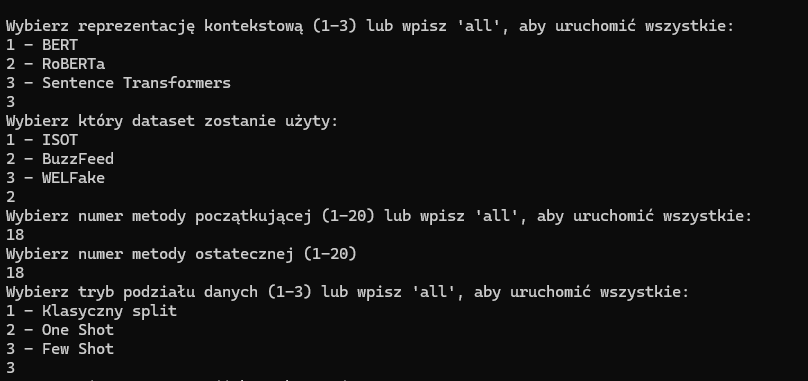
\includegraphics[scale=0.5]{img/app/console.png}
    \caption{Przykładowe uruchomienie aplikacji.}
    \label{fig:app_start_window}
\end{figure}

\subsection{Warstwa Oceny Wyników}
Ocena skuteczności modeli przeprowadzana jest za pomocą funkcji \texttt{evaluate\_model} z modułu \texttt{common.py}. Funkcja ta oblicza kluczowe metryki, w tym:
\begin{itemize}
    \item Dokładność (Accuracy),
    \item Precyzję (Precision),
    \item Recall,
    \item F1-Score,
    \item ROC-AUC,
    \item MCC,
    \item Log Loss,
    \item Cohen's Kappa.
\end{itemize}
Dodatkowo obliczane są metryki walidacji krzyżowej (CV Accuracy). Wyniki zapisywane są w osobnych plikach \texttt{runX\_dataset\_results.csv} i \texttt{runX\_dataset\_pr\_curve.csv} w folderach \texttt{results\_X\_Y}, gdzie \texttt{X} określa typ reprezentacji, a \texttt{Y} tryb podziału danych, przykładowo \texttt{results\_3\_few\_shot}. Każdy folder przechowuje wyniki specyficzne dla danego eksperymentu.

\subsection{Warstwa Wizualizacji}

Analiza graficzna wyników realizowana jest przez skrypt \texttt{all\_plots.py}, który przetwarza dane z plików CSV zapisanych w folderach \texttt{results\_X\_Y}. Generowane są:
\begin{itemize}
    \item Wykresy słupkowe porównujące metryki, takie jak Dokładność, Czas wykonania czy Log Loss oraz inne, dla różnych metod i zbiorów danych (BuzzFeed, ISOT, WELFake).
    \item Krzywe Precision-Recall dla każdej metody i zbioru danych.
\end{itemize}
Wykresy są zapisywane w folderze \texttt{plots}, zorganizowanym w podfoldery według datasetów i typów eksperymentów, co ułatwia ich przeglądanie.